%\chapter{EEPPI-Usermanual}
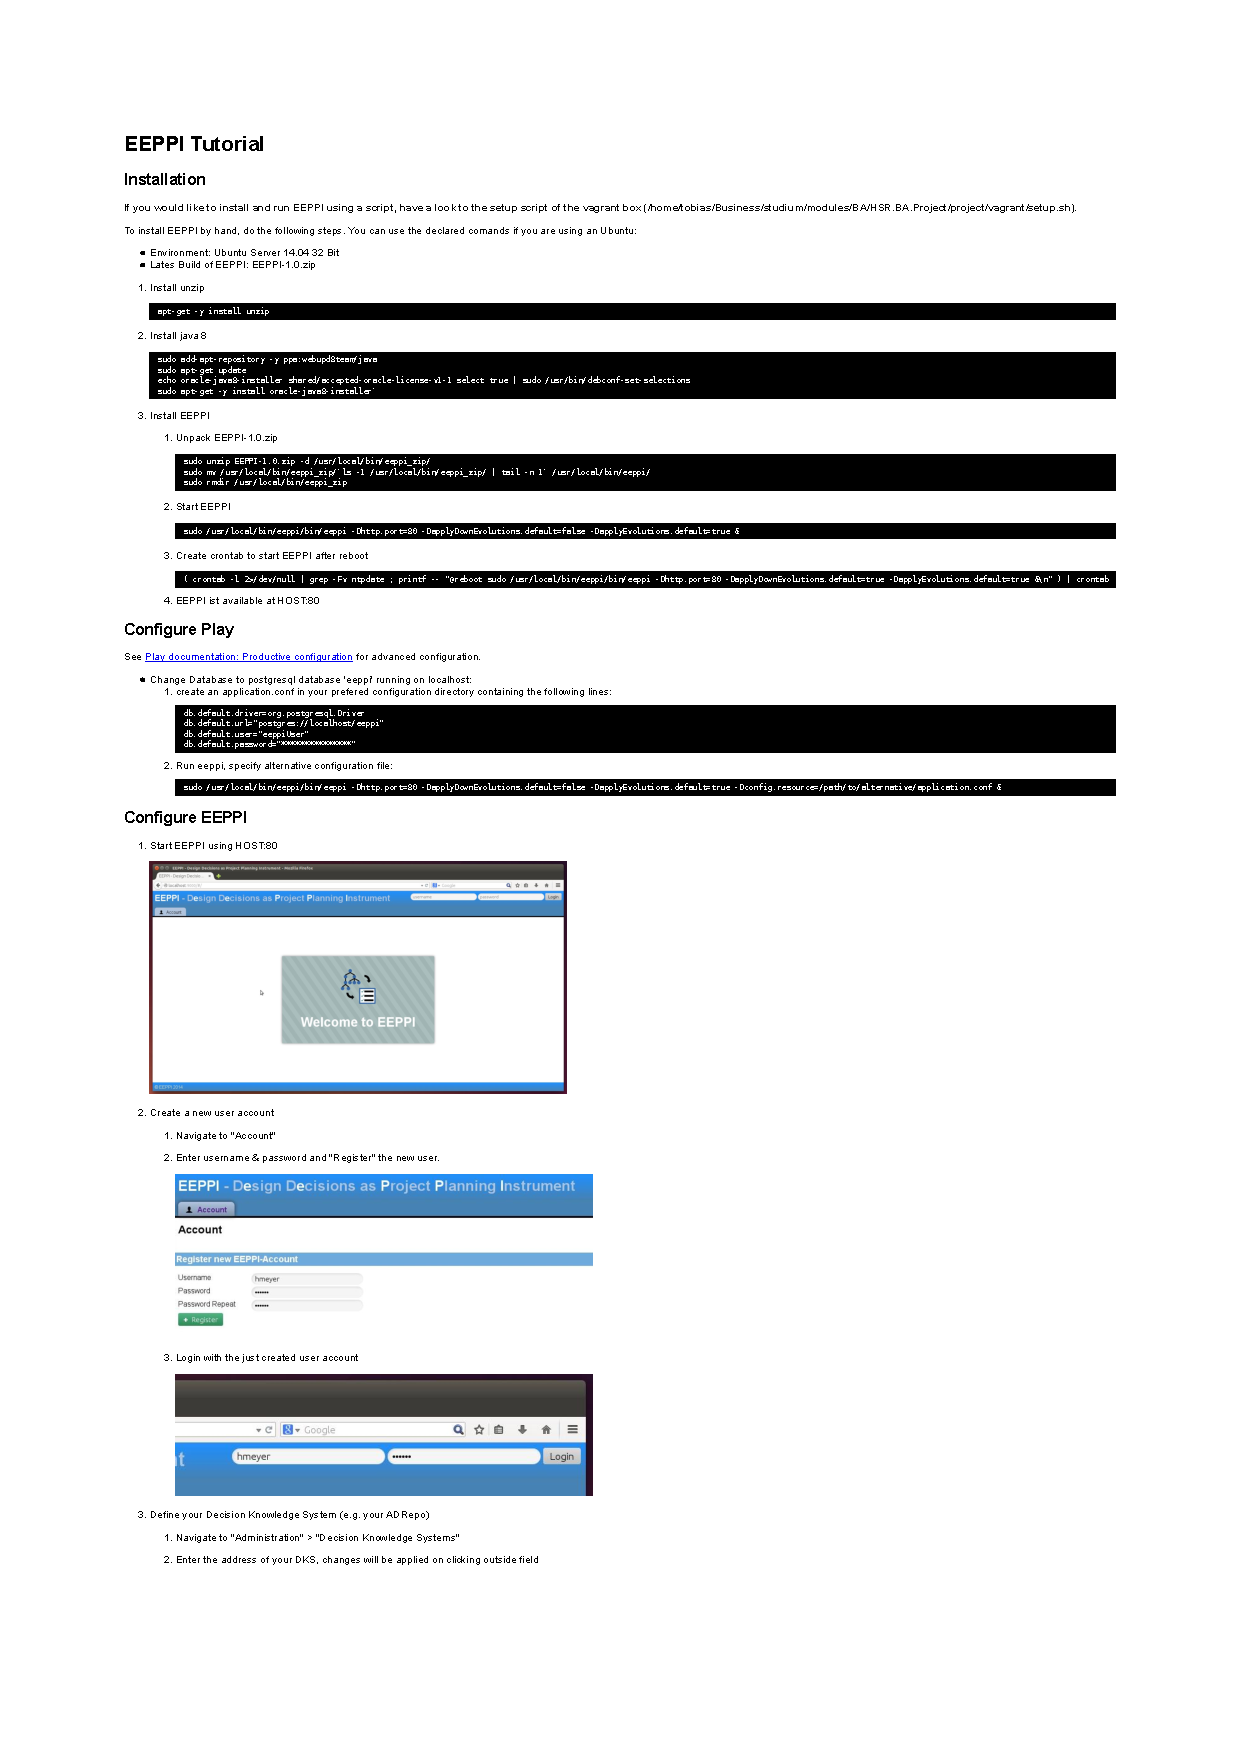
\includepdf[pages=-, pagecommand={},addtotoc={1,chapter,1,{EEPPI-Usermanual},chapter:userManual}]{tutorial/media/EEPPI-Usermanual.pdf}

\section{Beispieldaten für Request-Templates}
\label{sec:ExampleProcessorData}
	Wie im Usermanual beschrieben, braucht es ein Request-Template, um Tasks an ein \ppt\ zu übertragen.
	In Abbildung~\ref{fig:exampleRequestTemplate} ist ein Beispiel für ein Request-Template abgebildet, das gleiche ist auch im Usermanual zu finden.
	
	\begin{figure}[H]
		\begin{lstlisting}
{
	"issue": {
		"project_id": "${pptProject}",
		"tracker_id": $getTrackerByType:(taskTemplate.type)$,
		"subject": "${taskTemplate.name}",
		"assigned_to_id": $getAssigneeIdByName:(taskTemplate.attributes.Assignee)$
	}
}

		\end{lstlisting}
		\centering
		\caption{Beispiel eines Request-Tempaltes}
		\label{fig:exampleRequestTemplate}
	\end{figure}	
	
	In diesem Beispiel ist zu sehen, wie verschiedene Variablen verwendet werden.
	Es sind die folgenden Variablen verfügbar, sie sind auch im Usermanual beschrieben:
	\begin{itemize}
		\item taskTemplate
		\item node
		\item pptProject
		\item parentRequestData
	\end{itemize}
	Diese Variablen repräsentieren Objekte, beziehungsweise ganze Objektgraphen.
	Mittels dem Punkt-Operator kann durch durch diesen Graph navigiert werden.
	
	Nachfolgend wird ein Beispiel eines Objektgraphen gezeigt,
	um eine Vorstellung zu vermitteln, welche Daten verfügbar sind.

	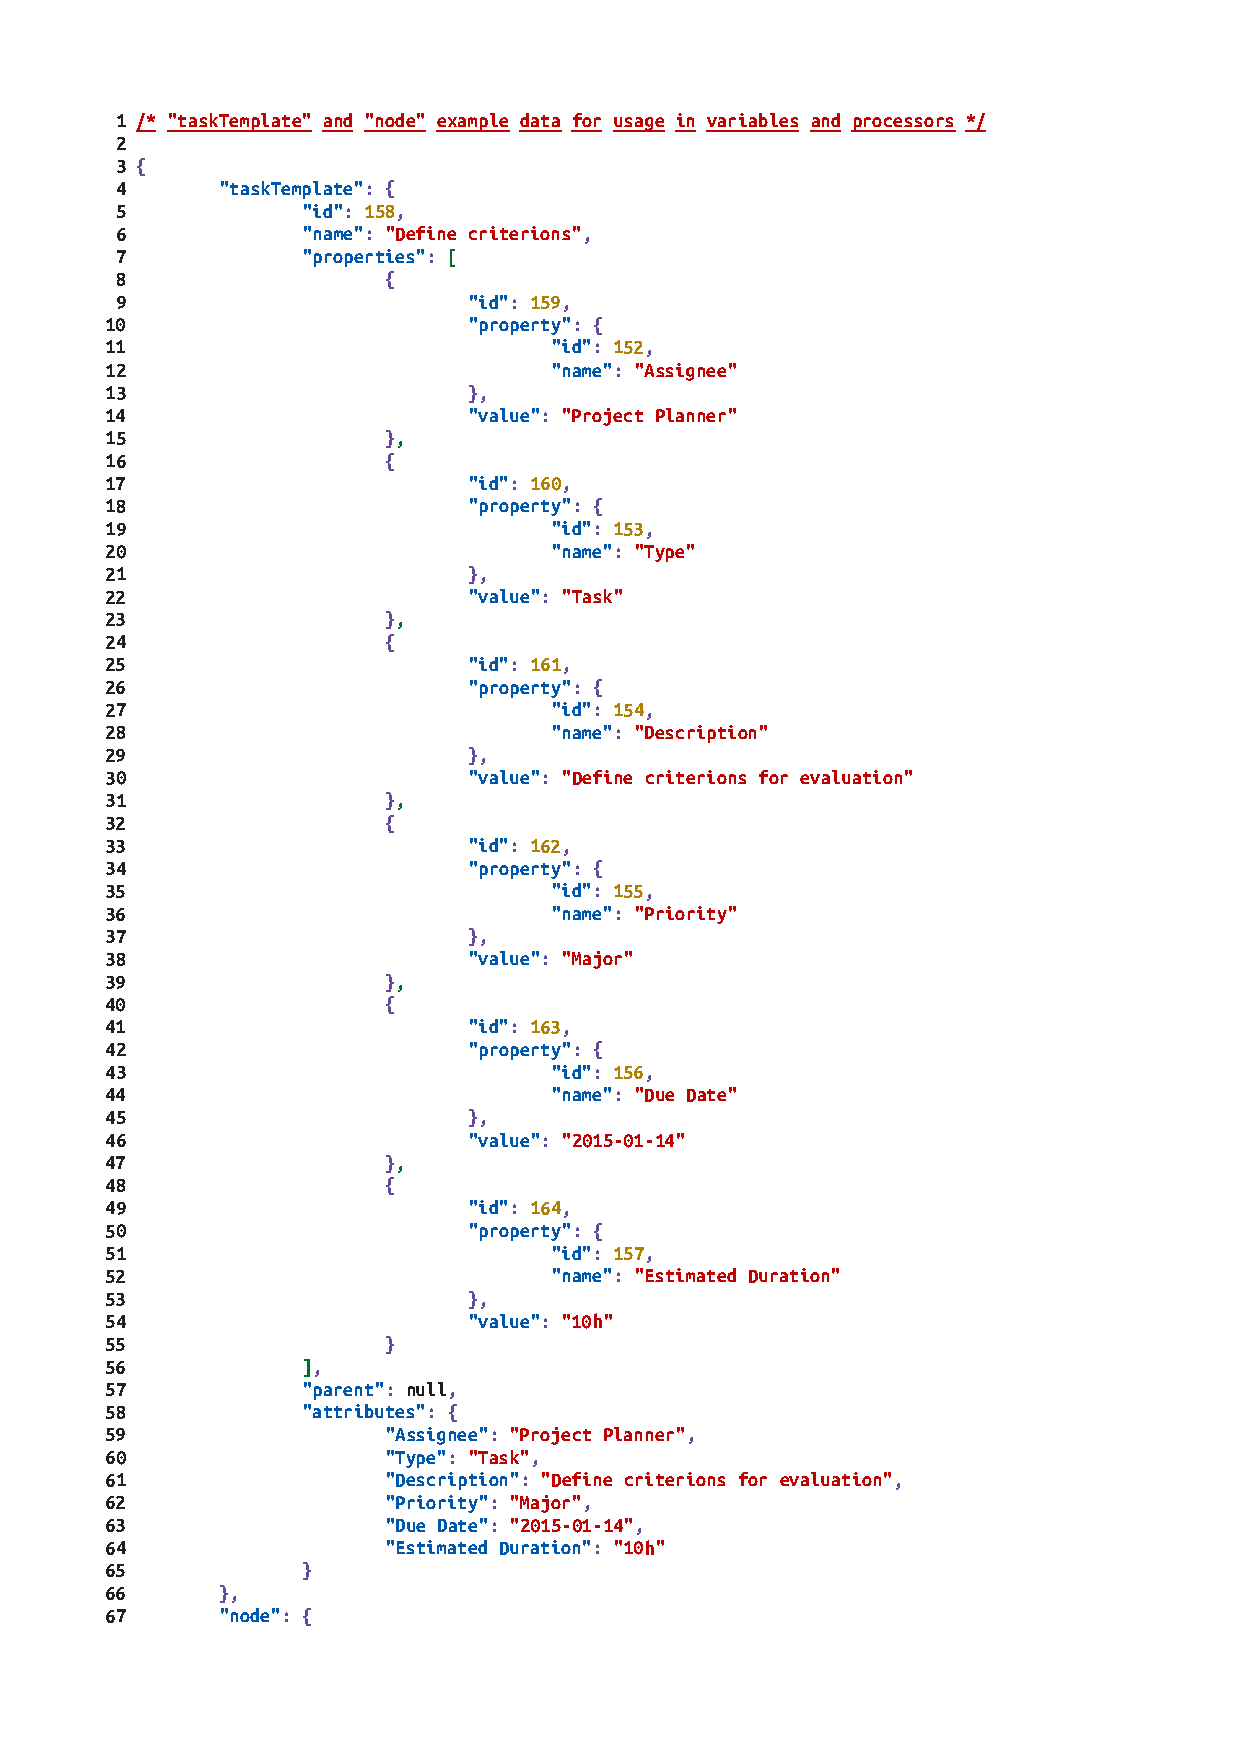
\includepdf[pages=-, pagecommand={}]{tutorial/media/requestTemplateVariablesExample.pdf}
